\section{Infinite-\texorpdfstring{$N$}{N} analysis of homogeneous phases}\label{sec:gnInfHomo}
\begin{disclaimer}
	This section follows the discussion presented in Sec. V of \ccite{Stoll:2021ori}.
	
	The results for the homogeneous phase diagram in \cref{fig:GNlargeN_PD} were obtained with my \Cpp{} code~\cite{Steil:2023GNcpp}, computing 39887 points in the $\mu$-$T$-plane in about an hour CPU time on an \ryzen{} processor (6 minutes wall time on 12 cores).
	The results of the Ginzburg–Landau analysis of the homogeneous phase diagram took only a few minutes to compute on an \intel{} with the \WAM{} notebook~\cite{Steil:2023GNnotebook}.
\end{disclaimer}
In this section, we will rediscover some of the well-known results for the infinite-$N$ (mean-field) limit of the \gnyBm{}.
We will demonstrate that the \frg{} in \lpa{} is capable of reproducing the latter results analytically and numerically.
Additionally, these mean-field calculations are used to motivate a proper \uv{} \ic{} for the flow equation \eqref{eq:pdeq-U} in \cref{subsec:UUV}, but also serve as a consistency check of our numerical implementation in the limit $N \rightarrow \infty$ in \cref{paragraph:numeric_consistency_check_mean-field}.

Within \cref{subsec:GNUvac} we will discuss the effective potential of the \gnyBm{} in vacuum and the related notion of asymptotic freedom in this context.
In \cref{subsec:phase_diagram_mean_field} we present results for the homogeneous phase diagram at infinite $N$.
We conclude this section with \cref{subsec:GNGL}, discussing the \gla{} for the \gnyBm{} and Landau’s theory of phase transitions.

\paragraph{Mean-field, infinite-\texorpdfstring{$N$}{N}, and FRG}\phantomsection\label{paragraph:mean-field_infinite_n_frg}\mbox{}\\%
Within the \frg{} framework (arguably even in general), the term ``mean-field approximation'' has no universal, agreed upon formal definition.
Usually performing calculations on ``mean-field level'' in the context of fermionic models refers to computations including only fermionic fluctuations, while disregarding bosonic ones.
Whether this includes fermionic vacuum fluctuations and/or fermionic contributions beyond the effective potential usually depends on the work under consideration.
In the \frg{} one way to define a mean-field approximation is the usage of a \lpa{} truncation disregarding the bosonic fluctuations.
This can be formally achieved by taking the infinite-$N$ limit for the \lpa{} flow equation under consideration, in this chapter \cref{eq:pdeq-U}, after appropriate rescalings, like the ones introduced in \cref{eq:rescaling_with_n}.
	
However, it can be shown that in general the infinite-$N$ limit and ``ignoring the bosonic loop in a \lpa{} truncation'' is not the same procedure. 
In fact, if starting with a more advanced \frg{} truncation scheme, like \lpap{}, which also includes wave-function renormalizations, one finds, that even in the infinite-$N$ limit, there are fermionic loop contributions to the bosonic wave-function renormalization, see, \eg{}, \ccite{Braun:2010tt,Braun:2011pp} and especially the corresponding discussion in \cref{subsec:stability}.
Hence, in general the order of ``limits'' plays a crucial role and ``choosing a truncation scheme in \frg{}'' and ``taking the infinite-$N$ limit'' do not necessarily commute.
We will also mention some subtleties when it comes to variants of the mean-field approximation in \cref{sec:cdwmf}.
Furthermore in models including Goldstone bosons/pions a large-$N$ limit for fermions, \eg{}, in the large-$N_f$ limit for chiral fermion flavors, does not lead to the desired suppression of bosonic modes{}, because the Goldstone modes{}/pions do not form as flavor singlets \dash{} pionic contributions to the \lpa{} flow equation are usually proportional to $N_f^2-1$, \cf{} \cref{eq:flow_equation_effective_potential}.
Another degree of freedom, \eg{}, the number of colors $N_c$, has to be used to facilitate the large-$N$ limit and the desired suppression of bosonic fluctuations.
	
For our purposes in this chapter, we simply start by definition on the level of the \lpa{} and take all limits like the infinite-$N$ limit or the zero-$T$ and zero-$\mu$ limit afterwards.
Hence, within our truncation, the mean-field limit and the infinite-$N$ limit are considered to be identical, which simplifies the discussion and allows to make direct contact with established conventional mean-field computations for the \gn{} model, \cf{} \ccite{Wolff:1985av,Thies:2006ti}, which consider only fermionic fluctuations on the level of the effective potential.\bigskip
	
Performing the large-$N$ limit for the flow equation \eqref{eq:pdeq-U}, yields
\begin{align}
	\lim\limits_{N \rightarrow \infty} \partial_t U ( t,  \sigma ) =\, & \frac{d_\gamma}{\piu} \, \frac{k^3 ( t )}{2 E_{\textrm{f}} ( t, \sigma )} \, \big( 1 - n_\mathrm{f} [ \beta ( E_{\textrm{f}} ( t, \sigma ) + \mu ) ] - n_\mathrm{f} [ \beta ( E_{\textrm{f}} ( t, \sigma ) - \mu ) ] \big) \, .\label{eq:pdeq-U-MF}
\end{align}
We find that the former \pde{} decouples in field space and reduces to a first-order \ode{} in $t$ at each point in $\sigma$-direction.
In the fluid-dynamic picture, on the level of $u ( t, \sigma ) = \partial_\sigma U ( t,  \sigma )$, this is rather intuitive, since the fermionic contribution to the flow equation \eqref{eq:pdeq-u} presents as a local time-dependent source/sink term \eqref{eq:source_sink} and the spatial movement of the fluid (via diffusion in field space) is totally suppressed.
On a mathematical and also technical level this changes and in fact simplifies the flow equation drastically.
We are no longer dealing with a non-linear parabolic \pde{} including a sink/source term, we are just left with a comparatively simple \ode{} which can be integrated directly.
The notion of irreversibility of \frg{} flows is completely lost in this limit.

When disregarding bosonic fluctuations completely in mean-field approximation all three model variants \dash{} \gn{}, \bgn{} and \gnym{} \dash{} introduced in \cref{subsec:gnyTmu} are equivalent. 
The \bgn{} and \gnym{} are identical in mean-field approximation and the \bgnm{} as the bosonized version of the \gnm{} is in general physically equivalent to the latter as already discussed in \cref{subsec:gnyTmu}.
This is the reason for us using the collective term \gnyBm{} so far in this section but for the remainder of the section we will just use the term \gnm{}.

\subsection{The mean-field vacuum potential and asymptotic freedom}\label{subsec:GNUvac}
Due to the decoupling in field space, the differential equation \eqref{eq:pdeq-U-MF} can be integrated analytically in $k ( t )$.
Using the definition of the \rgtime{} \eqref{eq:def_rg_time}, which implies $\partial_t = - k \, \partial_k$, we find
\begin{subequations}\label{eq:rg-U-MF}
\begin{align}
\newSubEqBlock
	U_{k=0}(\sigma) = \, & U_{k=\Lambda} (\sigma ) + \frac{d_\gamma}{\piu} \int_{0}^{\Lambda} \dif k \, \frac{k^2}{2 E_\mathrm{f}} \, \big( 1 - n_\mathrm{f} [ \beta ( E_\mathrm{f} + \mu ) ] - n_\mathrm{f} [ \beta ( E_\mathrm{f} - \mu ) ] \big) \,\equiv \\[.2em]
	U_{0}(\sigma) = \, & U_{\Lambda} (\sigma ) + \frac{d_\gamma}{\piu} \, \bigg[ \frac{k}{2} \, \big( E_\mathrm{f} + \tfrac{1}{\beta} \ln \big[ 1 + \eu^{- \beta ( E_\mathrm{f} + \mu )} \big] + \tfrac{1}{\beta} \ln \big[ 1 + \eu^{- \beta ( E_\mathrm{f} - \mu )} \big] \big) \bigg]_{0}^{\Lambda}\, - \nonumber\\*[.2em] % no page break
	& - \frac{d_\gamma}{2 \piu} \int_{0}^{\Lambda} \dif k \, \big( E_\mathrm{f} + \tfrac{1}{\beta} \, \ln \big[ 1 + \eu^{- \beta ( E_\mathrm{f} + \mu )} \big] + \tfrac{1}{\beta} \, \ln \big[ 1 + \eu^{- \beta ( E_\mathrm{f} - \mu )} \big] \big) \, ,
\end{align}
\end{subequations}
where the \uv{} \ic{} for this trivial integrable ``\frg{}-flow'' is given by the classical \uv{} potential, see \cref{paragraph:gnyVac},
\begin{align}
	U_{\Lambda}(\sigma)\equiv U ( t=0, \sigma ) = \tfrac{1}{2 g^2} \, ( h \sigma )^2	\label{eq:initial_potential}
\end{align}
and where we introduced the notation\footnote{%
This chapter does not share the at times lenient approach of \cref{sec:FRG,chap:zeroONSU2} when it comes to when, where, and how to denote \rg{}-scale- and -time-dependencies.
We will consistently use $U_k(\sigma)$ and $U(t,\sigma)$ \dash{} \ie{}, the given notation of \ccite{Stoll:2021ori}.
}
\begin{align}
	U_k(\sigma)\equiv U_{k(t)}(\sigma)\equiv U(t,\sigma) 
\end{align}
for the potential at a given \rgscale{} $k$ and the corresponding \rgtime{} $t$.
	
In the second line of \cref{eq:rg-U-MF} we integrated by parts in order to recover the usual expression for the grand canonical potential density for $\Lambda \rightarrow \infty$ (up to an infinite constant $\sim k \, E_\mathrm{f} \big|_{k = \Lambda}$), \cf{}\ \ccite{Harrington:1974tf,Jacobs:1974ys,Wolff:1985av,Thies:2006ti}.
The first terms of the integrands of \cref{eq:rg-U-MF} lead to divergences.
These divergences have to be canceled by ``renormalizing'' the coupling $g^2$ such that the \ir{} observables are finite and could in principle be matched with experimental observations.
The renormalized version of this so-called \textit{vacuum contribution} (the only contribution, that does not depend on $\mu$ and $T$) is directly linked to the \ic{} of our \frg{}-flows, when solving the \pde{} \eqref{eq:pdeq-U} and \ode{} \eqref{eq:pdeq-U-MF} (numerically), see \cref{subsec:UUV} and \cref{paragraph:numeric_consistency_check_mean-field}.
	
For renormalization, we turn to the $(\mu = 0)$- and $(\beta \rightarrow \infty\Leftrightarrow T\rightarrow 0)$-limit of \cref{eq:rg-U-MF},
\begin{align}
	U_{0;\mathrm{vac}} (\sigma ) \equiv \, & \lim\limits_{\mu,T \rightarrow 0} U_0 ( \sigma ) =	 \, \frac{h^2 \sigma^2}{2 g^2} + \frac{d_\gamma}{2 \piu} \int_{0}^{\Lambda} \dif k \, \frac{k^2}{\sqrt{ k^2 + h^2 \sigma^2 }} \, ,	\label{eq:ir_potential_mean-field_vac}
\end{align}
and study the corresponding gap equation
\begin{subequations} \label{eq:gapeq}
\begin{align}
	0 \overset{!}{=} \, & \frac{1}{h^2\sigma_0} \, \partial_{ \sigma} U_{0;\mathrm{vac}} (\sigma ) \big|_{ \sigma = \sigma_0} =	\,  \frac{1}{g^2} - \frac{d_\gamma}{2\piu} \int_{0}^{\Lambda} \dif k \, \frac{k^2}{( k^2 + h^2 \sigma_0^2 )^\frac{3}{2}} \\*[.1em] % no page break
	= \, & \frac{1}{g^2} + \frac{d_\gamma}{2 \piu} \, \bigg[ \frac{k}{\sqrt{ k^2 + h^2 \sigma_0^2 }} \bigg|_0^\Lambda - \int_{0}^{\Lambda} \dif k \, \frac{1}{\sqrt{ k^2 + h^2 \sigma_0^2 }}\bigg]	
	\\*[.1em] % no page break
	= \, & \frac{1}{g^2} + \frac{d_\gamma}{2 \piu} \, \bigg[ \Big[ 1 + \big( \tfrac{h \sigma_0}{\Lambda} \big)^2 \Big]^{- \frac{1}{2}} - \mathrm{artanh} \bigg( \Big[ 1 + \big( \tfrac{h \sigma_0}{\Lambda} \big)^2 \Big]^{- \frac{1}{2}} \bigg) \bigg] \,. 
\end{align}
\end{subequations}
at possible non-trivial minima $\sigma_0 \neq 0$, \cf{}\ \ccite{Rosenstein:1990nm,Wolff:1985av,Thies:2006ti}.
Hence, as a first result, assuming that $\sigma_0$ is non-zero and finite, we can study the asymptotic behavior of \cref{eq:gapeq} for $\Lambda \ggg h$,
\begin{align}
	\tfrac{1}{g^2} = \, & \tfrac{d_\gamma}{2 \piu} \, \big[ - 1 + \tfrac{1}{2} \ln \big( \big( \tfrac{2 \Lambda}{h \sigma_0} \big)^2 \big) \big] + \order \big( \big( \tfrac{h \sigma_0}{\Lambda} \big)^2 \big) \, .	\label{eq:asymptotics_of_g}
\end{align}
This reflects the asymptotically free behavior of the four-Fermi coupling~\cite{Gross:1974jv,ZinnJustin:2002ru,Peskin:1995ev} of the original Gross-Neveu model \eqref{eq:gn-model}, since
\begin{align}
	\lim\limits_{\frac{\Lambda}{h} \rightarrow \infty} g^2 = 0 \, .
\end{align}
Furthermore, we can use \eqref{eq:asymptotics_of_g} and solve for $\sigma_0$,
\begin{align}
	\sigma_0 = \pm \tfrac{2 \Lambda}{h} \, \eu^{- \frac{4 \piu}{d_\gamma g^2} -\frac{1}{2} } \, .
\end{align}
Hence, due to the asymptotic free behavior of $g^2$, there is \ZII{} (discrete chiral) symmetry breaking via two non-trivial minima for all non-zero $g^2$ in vacuum and for infinite-$N$ \dash{} a central result for the \gnm{}~\cite{Gross:1974jv}.

Furthermore, we can insert the results from the gap equation \eqref{eq:gapeq} in \cref{eq:initial_potential} and solve for the \uv{} potential
	\begin{align}
		U_\Lambda( \sigma ) = \, & \tfrac{d_\gamma}{4 \piu} \, ( h \sigma )^2 \, \bigg[ \mathrm{artanh} \bigg( \Big[ 1 + \big( \tfrac{h \sigma_0}{\Lambda} \big)^2 \Big]^{- \frac{1}{2}} \bigg) - \Big[ 1 + \big( \tfrac{h \sigma_0}{\Lambda} \big)^2 \Big]^{- \frac{1}{2}} \bigg] \, .		\label{eq:initial-condition}
	\end{align}
In the limit $\tfrac{\Lambda}{h} \to \infty$ we approach the Gaussian fixed point (\uv{} fixed point) for the \bgn{} model~\eqref{eq:bgn-model}, which becomes clear when considering dimensionless quantities
	\begin{align}
		&	\tilde h = \tfrac{1}{\Lambda} \, h \, ,	\qquad	\tilde{U}_\Lambda ( \sigma ) = \tfrac{1}{\Lambda^2} \, U_\Lambda (\sigma ) \, .	\label{eq:gaussian_fixed_point}
	\end{align}
Both, $\tilde{h}$ and $\tilde{U}_\Lambda (\sigma )$, vanish in the limit $\tfrac{\Lambda}{h} \to \infty$. This implies \dash{} as expected \dash{} that the \bgn{} model~\eqref{eq:bgn-model} in vacuum in the infinite-$N$ limit, is also asymptotically free.\bigskip

Turning now to the \ir{} mean-field potential \eqref{eq:ir_potential_mean-field_vac} and using the previous results, we find
\begin{align}
	 U_{0;\mathrm{vac}} ( \sigma )	= \, & \tfrac{d_\gamma}{4 \piu} \, ( h \sigma )^2 \, \bigg[ \mathrm{artanh} \bigg( \Big[ 1 + \big( \tfrac{h \sigma_0}{\Lambda} \big)^2 \Big]^{- \frac{1}{2}} \bigg) - \Big[ 1 + \big( \tfrac{h \sigma_0}{\Lambda} \big)^2 \Big]^{- \frac{1}{2}}\, - \nonumber \\*[.2em] % no page break
	&  \qquad\qquad\quad - \mathrm{artanh} \bigg( \Big[ 1 + \big( \tfrac{h \sigma}{\Lambda} \big)^2 \Big]^{- \frac{1}{2}} \bigg) \bigg] +	 \tfrac{d_\gamma}{4 \piu} \, \Lambda^2 \, \sqrt{1 + \big( \tfrac{h \sigma}{\Lambda} \big)^2 } \, .	\label{eq:U0vac}
\end{align}
Considering the first derivative of \cref{eq:U0vac} one can verify ${0=\partial_\sigma U_{0;\mathrm{vac}}( \sigma )|_{\sigma_0}}$ which has to hold by construction and we note that
	\begin{align}
		\partial_\sigma^2 U_{0; \mathrm{vac}} ( \sigma ) |_{\sigma_0} = \frac{d_\gamma}{2 \piu} \, \frac{\Lambda^3}{[ \Lambda^2 + ( h \sigma_0 )^2 ]^{3/2}} \, h^2, \label{eq:msigma_MF_Lambda}
	\end{align}
which is manifest positive \dash{} again consistent with the notion of $\sigma_0$ as a non-trivial minimum by construction \dash{} and corresponds to the squared curvature mass $m_\sigma^2$ of the \sigmaMode{} in vacuum.

Considering the limit $\tfrac{\Lambda}{h} \rightarrow \infty$ in \cref{eq:U0vac}, the divergent contributions of the two $\mathrm{artanh}$ cancel exactly. For the last term, we use
	\begin{align}
		\Lambda^2 \, \sqrt{1 + \big( \tfrac{h \sigma}{\Lambda} \big)^2} = \Lambda^2 + \tfrac{1}{2} \, ( h \sigma )^2 + \order \big( \big( \tfrac{h \sigma}{\Lambda} \big)^2 \big) \, ,
	\end{align}
which results in an unobservable infinite constant and a finite contribution.
In total we find the well-known renormalized vacuum \ir{} effective potential, \cf{} \ccite{Wolff:1985av,Thies:2006ti},
	\begin{align}
		U_{0;\mathrm{vac}} ( \sigma ) =	\, & \tfrac{d_\gamma}{8 \piu} \, ( h \sigma )^2 \, \big( \ln \big( \tfrac{h \sigma}{h \sigma_0} \big)^2 - 1 \big) + \tfrac{d_\gamma}{4 \piu} \, \Lambda^2 + \order \big( \big( \tfrac{h \sigma}{\Lambda} \big)^2 \big) \, ,	\label{eq:vacuum_potential}
	\end{align}
with its global minimum at $\pm\sigma_0$ and with a corresponding squared curvature mass of 
	\begin{align}
		m_\sigma^2 = \tfrac{d_\gamma}{2\piu} \, h^2 \, ,	\label{eq:msigma_MF}
	\end{align}
\cf{}\ \ccite{Gross:1974jv}. 

Finally, the result \eqref{eq:vacuum_potential} can be used to also simplify the full \ir{} potential in medium \eqref{eq:rg-U-MF} by replacing the vacuum contributions,
	\begin{align}
		U_0( \sigma ) = \, & \tfrac{d_\gamma}{8 \piu} \, ( h \sigma )^2 \, \big( \big[ \ln \big( \tfrac{h \sigma}{h \sigma_0} \big)^2 \big] - 1 \big) + \tfrac{d_\gamma}{4 \piu} \, \Lambda^2 + \order \big( \big( \tfrac{h \sigma}{\Lambda} \big)^2 \big)\, -\notag\\*% no page break
		&\qquad- \tfrac{d_\gamma}{2 \piu} \int_{0}^{\Lambda} \dif p \, \big(\tfrac{1}{\beta} \, \ln \big[ 1 + \eu^{- \beta ( E_\mathrm{f} + \mu )} \big] + \tfrac{1}{\beta} \, \ln \big[ 1 + \eu^{- \beta ( E_\mathrm{f} - \mu )} \big] \big) \, .\label{eq:medium_potential}
	\end{align}
For $\Lambda \rightarrow \infty$ we can read off from \cref{eq:vacuum_potential} that the model contains only a single internal dimensionful parameter, for instance $h$, because the bosonic field $\sigma$ is dimensionless and $h$ and $\sigma$ only appear in combination. 
All other dimensionful quantities ($\mu$, $T$, $\Lambda$, $U$) can be expressed via this single parameter and results for different specifications of the reference parameter can be mapped into each other via simple rescaling.
A direct consequence is that also the mean-field phase diagram is unique, as is discussed in the next \cref{subsec:phase_diagram_mean_field}.

\subsection{The mean-field phase diagram in the renormalized limit \texorpdfstring{$\Lambda\rightarrow\infty$}{}}
\label{subsec:phase_diagram_mean_field}
In this subsection we will discuss the mean-field potential $U_0 ( \sigma )$ of \cref{eq:medium_potential} in the limit $\Lambda\rightarrow\infty$.
We will compare our analytical results of this subsection with the existing renormalized mean-field results of specifically \ccite{Wolff:1985av,Thies:2006ti} for the Gross-Neveu model at vanishing bare fermion mass.
Of special interest is the phase-diagram (see Figure~1 of \ccite{Thies:2006ti} or Fig.~3 of the preceding publication~\cite{Wolff:1985av}) and the underlying renormalized grand canonical potential density, see, \eg{}, Eq.~(4) of \ccite{Thies:2006ti}.
The results of this section will serve as a reference in the consistence check of our numerical implementation in \cref{paragraph:numeric_consistency_check_mean-field}.\bigskip

Consider the mean-field potential $U_0(\sigma)$ of \cref{eq:medium_potential} in the renormalized limit $\Lambda\rightarrow\infty$,

\begin{align}
	\lim_{\Lambda \rightarrow \infty} U_0(\sigma) - \tfrac{d_\gamma }{4\piu} \, \Lambda^2\, &=\, \tfrac{d_\gamma}{8 \piu} \, ( h \sigma )^2 \, \big( \ln \big[ \big( \tfrac{h \sigma}{h \sigma_0} \big)^2 \big] - 1 \big)\,- \notag \\* % no page break
	&\qquad - \tfrac{d_\gamma}{4 \piu} \int_{-\infty}^{+\infty} \dif k \, \big( \tfrac{1}{\beta} \, \ln \big[ 1 + \eu^{- \beta ( E_\mathrm{f} + \mu )} \big] + \tfrac{1}{\beta} \, \ln \big[ 1 + \eu^{- \beta ( E_\mathrm{f} - \mu )} \big] \big) \, ,		\label{eq:rg-U-MF-largeLambda}
\end{align}
where we used the symmetry ($k \rightarrow - k$) of the remaining integral.
We identify several noteworthy terms in \cref{eq:rg-U-MF-largeLambda}:

\begin{itemize}
	\item the remaining integral is the canonical one-loop, convergent medium contribution of fermions in \dimPlus{1}{1} dimensions, \cf{} \cref{eq:VfmedApp},
	\item the vacuum contribution carries a, for $1 + 1$ dimensions typical~\cite{Actor:1985vh,Actor:1985xp,Actor:1986zf}, term proportional to $( h \sigma )^2 \, \ln ( h \sigma )$,
	\item and we subtracted a (in $\sigma$, $\mu$ and $\beta$) constant but otherwise divergent contribution proportional $\Lambda^2$ to perform the limit $\Lambda \rightarrow \infty$.
	In observables this divergent but constant contribution cancels (since $U_0(\sigma)$ is only defined up to a constant) and therefore it can be subtracted from $U_0(\sigma)$ without further consequences.
\end{itemize}
For the following we therefore consider the effective potential
	\begin{align}
		\VeffArgs{\muT;\sigma}\equiv \, & \lim_{\Lambda \rightarrow \infty} U_0(\sigma) - \tfrac{d_\gamma }{4\piu} \, \Lambda^2  =
	 \tfrac{1}{4 \piu} \, \sigma^2 \, \left[ \ln( \sigma^2 ) - 1 \right] + \VeffArgs[\mathrm{f};\med]{\muT;\sigma} \label{eq:rgMFV}
	\end{align}
where we used $d_\gamma=2$ as well as \wlogA{} $h = 1$ and $\sigma_0 = 1$ and abbreviate the medium contribution with 
\begin{align}
	\VeffArgs[\mathrm{f};\med]{\muT;\sigma} \equiv \, & - \tfrac{T}{2 \piu} \int_{-\infty}^{+\infty} \dif k \, \ln \big[ 1 + \eu^{- \tfrac{1}{T} ( E_\mathrm{f} + \mu )} \big] - \tfrac{T}{2 \piu} \int_{-\infty}^{+\infty} \dif k \, \ln \big[ 1 + \eu^{- \tfrac{1}{T} ( E_\mathrm{f} - \mu )} \big] \, .
\end{align}

For a given $\mu$ and $T$ the physical value of the condensate $\sigma$ is found by minimization of $\VeffArgs{\muT;\sigma}$, according to \cref{paragraph:GNdSB}, \cref{app:grandCanonicalPartitionFunction}, and especially the discussion surrounding \cref{eq:VeffFdef}.
When evaluated at its global minimum $\VeffArgs{\muT;\sigma}$ is the renormalized grand canonical potential per spatial volume $\thermalGrandPotentialDensity$, \cf{} \cref{eq:thermalGrandPotentialDensity}.
The renormalized (\frg{}) mean-field result of \cref{eq:rgMFV} for $\VeffArgs{\muT;\sigma}$ obtained in the infinite-$N$ limit of the \lpa{} flow equation with a one-dimensional \lpa{}-optimized regulator \eqref{eq:pdeq-U-MF} coincides with the renormalized mean-field results in literature, see, \eg{}, \ccite{Wolff:1985av,Thies:2006ti}, and explicitly Eq.~(4) of \ccite{Thies:2006ti}.
In the rest of this subsection we derive and recapitulate known \mf{} results for the homogeneous phase diagram of the \gnm{}, see, \eg{}, \ccite{Wolff:1985av,Thies:2006ti}.\bigskip

\customWidthFigure%
	[!t]%
	{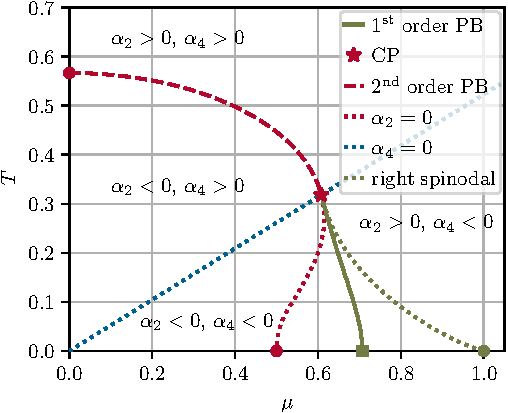
\includegraphics[width=7cm]{gn/figures/GNlargeN_PD.pdf}}% Graphics
	[]% Sublabels
	{%
		Phase diagram of the renormalized \gnm{} in the infinite-$N$ limit. The critical point (red star) separates the second-order phase boundary (red-dashed line) from the first-order phase boundary (solid green line). The red-dotted line and the green-dotted line are the left and right spinodal lines. 
		The {blue}\ ($\alpha_4=0$) and  {red}\ ($\alpha_2=0$) lines are obtained from the Ginzburg-Landau expansion of \cref{subsec:GNGL}. 
		The critical temperature $T_\mathrm{C}$ is marked on the $T$-axis with a red disk, while the end points at $\mu_\mathrm{L}$ and $\mu_\mathrm{R}$ of the spinodal lines are marked on the $\mu$-axis with red and green disks respectively. The first-order phase transition at zero temperature is marked with a green square at $\mu_1$.
		\fromFig{2}{Stoll:2021ori}
	}%Caption
	{fig:GNlargeN_PD}%Label

The phase diagram of \cref{fig:GNlargeN_PD} identical to the one presented in Fig.~1 of \ccite{Thies:2006ti}. 
The first-order phase boundary and the right spinodal have been obtained by explicit numerical integration~\cite{cubature:2020} and subsequent repeated, local, numerical minimization~\cite{Nelder:1965} of the renormalized grand canonical potential per spatial volume \eqref{eq:rgMFV} using my \Cpp{} code~\cite{Steil:2023GNcpp}.
The phase boundaries and the spinodal region have been obtained with the help of a block-structured adaptive mesh refinement algorithm, which I implemented for the efficient computation of phase diagrams and the precise detection of lines of interest, without the need of explicit bisection.
Details can be found in the \Cpp{} code~\cite{Steil:2023GNcpp} and its documentation \dash{} including a very instructive example using the Mandelbrot set \dash{} and in my group seminar talk~\cite{Steil:2020bsam}.

By construction \dash{} due to the renormalization condition of \cref{eq:gapeq} \dash{} discrete chiral symmetry is broken with $\sigma=\sigma_0=1$ in the vacuum at $T=\mu=0$.
At high chemical potentials and temperatures the discrete chiral symmetries is restored and therefore $\sigma=0$.
At intermediate temperatures and chemical potentials one observes a first-order phase transition line starting at zero temperature and non-zero chemical potential $\mu_1$ and ending in a critical point at $( \mu_{\mathrm{CP}}, T_{\mathrm{CP}} )$.
Above $T_{\mathrm{CP}}$ discrete chiral symmetry is restored across a second-order phase transition line starting at the critical point and ending on the $(\mu=0)$-axis at a non-zero temperature $T_\mathrm{C}$.

The position of the critical point $(\mu_{\mathrm{CP}},T_{\mathrm{CP}})$ as well as $\mu_\mathrm{L}$, $\mu_1$, $\mu_\mathrm{R}$, and $T_\mathrm{C}$ can be computed with the help of known functions without the need of numerical minimization of the potential $\VeffArgs{\muT;\sigma}$.
The determination of the location of the critical point and the value for the critical temperature will be discussed in the next \cref{subsec:GNGL}.
We devote the remainder of this subsection to considerations at zero temperature.

For $T \rightarrow 0$ the integral in $\VeffArgs[\mathrm{f};\med]{\muT;\Delta}$ can be performed analytically \dash{} as discussed in \cref{app:zeroT} \dash{} with the result
\begin{align}
	\VeffArgs[\mathrm{f};\med]{\mu,0;\sigma}=&	\tfrac{1}{2\piu} \, \Big( \sigma^2 \, \mathrm{arsinh} \Big[ \sqrt{ \big( \tfrac{\mu}{\sigma} \big)^2 - 1 } \Big] -\mu^2 \, \sqrt{1 - \big( \tfrac{\sigma}{\mu} \big)^2 } \,\Big) \, \Theta \big[ \big( \tfrac{\mu}{\sigma} \big)^2 - 1 \big] \, ,	\label{eq:rgMFIT0}
\end{align}
\cf{} \cref{eq:Vs1fmedT0App}, with $\Delta\equiv h \sigma$ and $h=1$ in the present setting.
We note $\VeffArgs[\mathrm{f};\med]{0,0;\sigma} = 0$ as all vacuum contributions are already integrated out and included in \cref{eq:rgMFV}.
An analysis of \cref{eq:rgMFIT0} reveals, that the extremum at $\sigma = 0$ becomes a local minimum for $\mu > \mu_\mathrm{L} = \tfrac{1}{2}$.
The potential has only a trivial minimum at $\sigma = 0$ for $\mu > \mu_\mathrm{R} = 1$.
For ${\mu \in [ \mu_\mathrm{L}, \mu_\mathrm{R} ]}$ the potential has three minima (one at $\sigma = 0$ and two at $\sigma = \pm 1$) and at $\mu_1 = \tfrac{1}{\sqrt{2}} \simeq 0.707107$ all local minima become global minima signaling a first-order phase transition at $\mu_1$.
The notable chemical potentials $\mu_\mathrm{L}$, $\mu_1$ and $\mu_\mathrm{R}$ are marked on the $(T=0)$-axis in \cref{fig:GNlargeN_PD}.

\subsection{Ginzburg-Landau analysis and Landau’s theory of phase transitions}\label{subsec:GNGL}
We will conclude our discussion of the homogeneous phase diagram of the \gnm{} in the infinite-$N$ limit by considering a \acrrepeat{gl} expansion/analysis of the effective potential $\VeffArgs{\muT;\sigma}$ of \cref{eq:rgMFV}.
A \gla{} in this context is an expansion of $\VeffArgs{\muT;\sigma}$ around $\sigma=0$, resulting in a Ginzburg–Landau type theory/potential~\cite{Ginzburg:1950sr}.
Details on such expansions in the context of theoretical physics can be found in, \eg{}, \ccite{\glRefs}.
We will use this expansion to comment on first and second-order phase transitions in the spirit of Landau’s theory of phase transitions~\cite{Landau:1937obd}.
A discussion of the latter in the context of the zero-dimensional theories of \cref{chap:zeroONSU2} can be fund in App.~B of \nbccite{zerod1}.
We have decided to not include this part of our studies in zero dimensions in favor of the present discussion, which is much more illuminating for the applications of this chapter and the next \cref{chap:QMM}.\bigskip

For the medium part $\VeffArgs[\mathrm{f};\med]{\muT;\sigma}$ of \cref{eq:rgMFIT0} a \gla{} is discussed in \cref{app:seriesV} with the relevant results in one spatial dimensions listed in \cref{app:Vmedf1Series} and specifically \cref{eq:s1alpha0,eq:s1alpha2,eq:s1alpha4,eq:s1alpha6}.
Note that these results are also included and in fact derived in the digital auxiliary \WAM{} notebook~\cite{Steil:2023PhDThermodynamicsNB}, which also includes the code employed in chapter 2 of the \WAM{} notebook~\cite{Steil:2023GNnotebook}, used to create the plots and results of this subsection.
For the discussion in this subsection we will adopt the notation of \cref{app:seriesV} and discuss the effective potential as a function of the fermion mass term $\Delta=\sigma h$.
For the remainder of this subsection all dimensionful quantities are assumed to be expressed in multiples of the fermion mass term in vacuum $\Delta_0\equiv h \sigma_0$ which has dimensions of energy.
We consider an expansion up to at most order six, \viz{}
\begin{align}
	\VeffFArgs[][(6)]{\muT;\Delta}=\sum_{m=0}^3\alpha_{2m}(\muT)\Delta^{2m}\,,\label{eq:GNgl}
\end{align}
with $\alpha_{2m}(\muT)=\alpha_{2m}^{s=1}(\muT)$. For $2m\in\{0,4,6\}$ explicit expressions can be found in \cref{eq:s1alpha0,eq:s1alpha4,eq:s1alpha6}.
$\alpha_{2}(\muT)$ gains a vacuum contribution from \cref{eq:vacuum_potential} additional to the medium contribution $\alpha_{2}^{(s=1)}(\muT)$ from \cref{eq:s1alpha2} and thus reads
\begin{align}
\alpha_{2}(\muT) = -\frac{1}{4\piu} + \frac{1}{2\piu}\ln\Delta +\alpha_{2}^{(s=1)}(\muT)\,,
\label{eq:GNalpha2}
\end{align}
where the $(\ln\Delta)$-term of the vacuum contribution cancels with the potential \ir{} divergence \dash{} in form of exactly such a $(\ln\Delta)$-term \dash{} in $\alpha_{2}^{(s=1)}(\muT)$. 

The expansion \eqref{eq:GNgl} around $\sigma = 0$ can be used to compute the second-order phase-boundary in terms of known functions including the critical point. The second-order phase transition between the restored and a broken phase with small $\sigma > 0$ occurs at $\alpha_2 = 0$ while $\alpha_4 > 0$. In the vicinity of a second-order phase transition one finds $\alpha_2 > 0$ and $\alpha_4 > 0$ in the restored phase while $\alpha_2 < 0$ and $\alpha_4 > 0$ holds in the broken phase in this context. Using \cref{eq:GNalpha2,eq:s1alpha2} we find the transition temperature at $\mu=0$
	\begin{align}
		T_\mathrm{C} = \frac{\eu^\emc}{\piu} \simeq 0.566933 \, .\label{eq:Tc_MF}
	\end{align}
The curvature $\kappa$ of the second-order phase boundary $T_\mathrm{C} \big( \tfrac{\mu}{T} \big) = T_\mathrm{C} \, \big[ 1 - \kappa \, \big( \tfrac{\mu}{T} \big)^2 + \ldots \big]$ at $\mu = 0$ can be computed using \cref{eq:s1alpha2} and is given by ${\kappa=\tfrac{7\zeta(3)}{4\piu^2} \simeq 0.213139}$.
For comparison recall $\kappa'=0.1584(9)$ from \cref{eq:kappaQCD} for $N_f=2$ \qcd{}.

The critical point is located at the intersection of the $\alpha_2 = 0$ and $\alpha_4 = 0$ lines, see, \eg{}, Refs.~\cite{Buballa:2014tba,Buballa:2018hux}.

Using \cref{eq:s1alpha4}, we determine $\tfrac{\mu_\mathrm{CP}}{T_\mathrm{CP}} \simeq 1.910669$ from the only root $z_{2,1}$ of $\mathrm{DLi}_{2}(z)$ from \cref{eq:DLi2Zero1}.
Having the ratio $\tfrac{\mu_\mathrm{CP}}{T_\mathrm{CP}}$ fixed, we determine
\begin{align}
	(\mu_\mathrm{CP}, T_\mathrm{CP} ) \simeq ( 0.608221, 0.318329 ) \, ,\label{eq:muCPTCP_MF}
\end{align}
using \cref{eq:GNalpha2}.
Above $T_\mathrm{CP}$ we have the second-order phase transition with $\alpha_4 > 0$, while below $T_\mathrm{CP}$ we have the spinodal region with $\alpha_4 < 0$ and $\alpha_6 > 0$ in the vicinity of the critical point. 
$\alpha_2 > 0$, $\alpha_4 < 0$, and $\alpha_6 > 0$ allows for three local minima in the Ginzburg-Landau potential \eqref{eq:GNgl} when considered up to $m = 3$, which indicates a first-order phase transition below $T_\mathrm{CP}$.
At the critical point ($\alpha_2 = \alpha_4=0$ and $\alpha_6 > 0$) the non-trivial minima from the ($\alpha_2 > 0$, $\alpha_4 < 0$)-scenario and ($\alpha_2 < 0$, $\alpha_4 > 0$)-scenario merge in $\sigma = 0$.
The $\alpha_2 = 0$ line below $T_\mathrm{CP}$ signals the appearance of a local minimum at $\sigma = 0$ and is called the left spinodal line ending in $\mu_\mathrm{L}$ at $T = 0$, in accordance with the results at $T = 0$ discussed earlier in the previous \cref{subsec:phase_diagram_mean_field}. 
The $\alpha_2=0$ and $\alpha_4=0$ lines are displayed in \cref{fig:GNlargeN_PD}.

Before discussing Landau’s theory of phase transitions in the present context in the next paragraph, we will comment on the \gle{} up to order $m=3$ and the corresponding results for the first-order phase-boundary and the right spinodal line.
In the following discussion the dimensionless ratio
\begin{align}
\eta_2\equiv \frac{\alpha_2 \,\alpha_6}{\alpha_4^2}\,,
\label{eq:GLeta2}
\end{align}
will be particularly useful.
A simple curve discussion of $\VeffArgs[][(6)]{\muT;\Delta}$ of \cref{eq:GNgl}, see subsection 5.1 of \ccite{Steil:2023PhDThermodynamicsNB}, reveals a spinodal region for $1-3\eta_2>0$, \ie{}, $\mathcal{V}^{(6)}$ develops five extrema in $\Delta$.
$\eta_2=\frac{1}{3}$ marks the right spinodal line.
Further analysis reveals that at $\eta_2=\frac{1}{4}$ the non-trivial minima at $\Delta=\pm\frac{|\alpha_4|}{2\alpha_6}$ become global minima, signaling a first-order phase transition at that point.

\fullWidthFigure%
	[!t]%
	{gn/figures/gn_gl_comp.pdf}% Graphics
	[fig:GNGLcompL,fig:GNGLcompS]% Sublabels
	{%
		Phase diagram of the renormalized \gnm{} in the infinite-$N$ limit based on the \gle{} with the right figure \subref{fig:GNGLcompS} being just a zoom-in (marked on the left \subref{fig:GNGLcompL} with a gray rectangle) around the \cp{}.
		The black lines are the numerical reference lines from \cref{fig:GNlargeN_PD} with the finite resolution of $0.1\cdot 2^{-7}=7.8125\cdot 10^{-4}$ in both $\mu$ and $T$ visible on the right.
		The \gl{} phase boundaries and lines are marked in the figure caption including their defining equation in the \gle{}. 
		The transparent purple dots are relevant for the \customref{paragraph:landauPTs}{following discussion} of phase transitions.
	}%Caption
	{fig:GNGLcomp}%Label
We are now in a position to compute the full \gl{}-based phase diagram by means of simple contour plots~\cite{Steil:2023PhDThermodynamicsNB}.
In \cref{fig:GNGLcomp} we confront the results of the \gle{} with the numerical results of \cref{fig:GNlargeN_PD}. 
Unsurprisingly we find a perfect agreement for the second-order phase boundary, the left spinodal line, and the critical point, since for those the \gle{} is perfectly justified.
For the first-order phase transition and right spinodal line we find a good agreement in the immediate vicinity around the critical point and quickly loose predictive power as we approach $\mu/T=z_{4,2}\simeq 4.359$, where $\alpha_6$ becomes negative and the expansion based on $\mathcal{V}^{(6)}$ breaks down.
It should however be stressed that around the critical point the \gle{} has booth qualitative and also quantitative power for both first- and second-order phase transitions.

\paragraph{Landau’s theory of phase transitions}\phantomsection\label{paragraph:landauPTs}\mbox{}\\%
\fullWidthFigure%
	[!t]%
	{gn/figures/gn_gl_1st_U.pdf}% Graphics
	[fig:GNGL2ndU,fig:GNGL1stU,fig:GNGL2ndmin,fig:GNGL1stmin]% Sublabels
	{%
		$\VeffArgs[][(4)]{0,T;\Delta}$ in \subref{fig:GNGL2ndU} and corresponding evolution of its minima in temperature in  \subref{fig:GNGL2ndmin}.
		$\VeffArgs[][(6)]{\mu,0.25;\Delta}$ in \subref{fig:GNGL1stU} and corresponding evolution of its minima in chemical potential in  \subref{fig:GNGL1stmin}.
		The extrema of the potentials are marked as dots in \subref{fig:GNGL2ndU} and \subref{fig:GNGL1stU}.
		The colors change from lower temperatures/chemical potentials in blue to higher ones in red.
	}%Caption
	{fig:GNGLUmin}%Label
In the following we will discuss second- and first-order phase transitions using the \gl{} effective potentials to fourth- and sixth-order ($\VeffArgs[][(4)]{\muT;\Delta}$ and $\VeffArgs[][(6)]{\muT;\Delta}$) respectively.
This discussion is based on the websites~\cite{Hadley:2022II,Hadley:2022I}, which not only provide an excellent explanation of Landau’s theory of phase transitions but also interactive tools to study them. 
We adapted the discussion of \ccite{Hadley:2022II,Hadley:2022I} to the \gn{} model at infinite $N$.
To discuss second-order phase transitions we follow the phase diagram at $\mu=0$ across the second-order phase transition.
To discuss first-order phase transitions we track through the spinodal region at a constant temperature $T=0.25$.
The respective relevant points for the following discussion are marked in \cref{fig:GNGLcomp} in purple.

In \cref{fig:GNGL2ndU,fig:GNGL2ndmin} we can observe symmetry restoration across a second-order phase transition, where the order parameter changes smoothly from $\Delta^2>0$ to $\Delta^2=0$.
As we approach $T_\mathrm{C}$ from below, the non-trivial minima located at $\Delta^2=-\frac{\alpha_2}{2\alpha_4}$ (note that $\alpha_2<0$ in the broken phase) melt away, \ie{}, they continuously merge into $\Delta=0$ as we approach $\alpha_2=0$ at the second-order phase boundary.

In \cref{fig:GNGL1stU,fig:GNGL1stmin} we can observe symmetry restoration across a first-order phase transition, where the order parameter changes discontinuously from $\Delta^2>0$ to $\Delta^2=0$.
The spinodal region, where five extrema and three minima coexist, is clearly visible in \cref{fig:GNGL1stU}.
At the first-order phase boundary the three minima (at $\Delta=0$ and $\Delta=\pm\frac{|\alpha_4|}{2\alpha_6}$) become degenerate and a discontinuous jump in $\Delta$ from the broken to the restored phase takes place.\bigskip
\fullWidthFigure%
	[!t]%
	{gn/figures/gn_gl_thermo1.pdf}% Graphics
	[fig:GNGL2ndf,fig:GNGL1stf,fig:GNGL2nds,fig:GNGL1sts,fig:GNGL2ndcv,fig:GNGL1stcv]% Sublabels
	{%
		Landau free energy density $f$, the entropy density $s$, and volumetric heat capacity $c_v$ across the second-order (first-order) phase transition in \subref{fig:GNGL2ndf}, \subref{fig:GNGL2nds}, and \subref{fig:GNGL2ndcv} (\subref{fig:GNGL1stf}, \subref{fig:GNGL1sts}, and \subref{fig:GNGL1stcv}) respectively plotted over temperature $T$ at $\mu=0$ (chemical potential $\mu$ at $T=0.25$).
	}%Caption
	{fig:GNGLfscv}%Label
This dynamics in the effective potential also imprints itself into thermodynamic observables.
Using the expressions provided in \cref{app:grandCanonicalPartitionFunction}, \ie{}, \cref{eq:thermalFreeEnergyDensity,eq:thermalEntropyDensity,eq:thermalNumberDensity}, we can compute
the Landau free energy density $f$, the entropy density $s$, and the mean quark number density $n$ with
\begin{align}
f=\VeffArgs{\muT;\Delta_\mathrm{min}}\, ,\qquad s = -\del{\frac{\partial f}{\partial T}}_\mu\, ,\qquad n = -\del{\frac{\partial f}{\partial \mu}}_T\,.
\end{align}
\fullWidthFigure%
	[!t]%
	{gn/figures/gn_gl_thermo2.pdf}% Graphics
	[fig:GNGL2ndn,fig:GNGL1stn,fig:GNGL2ndchiq,fig:GNGL1stchiq]% Sublabels
	{%
	 Mean quark number-density $n$ and quark number susceptibility $\chi_q$ across the second-order (first-order) phase transition in \subref{fig:GNGL2ndn} and \subref{fig:GNGL2ndchiq} (\subref{fig:GNGL1stn} and \subref{fig:GNGL1stchiq}) respectively plotted over temperature $T$ at $\mu=0$ (chemical potential $\mu$ at $T=0.25$). Note that $\chi_q$ is not the slope of $n$ in the $T$ direction but in $\mu$ direction.
	}%Caption
	{fig:GNGLfnchiq}%Label
Additionally we consider the first moments of entropy and mean quark number-density, \viz{} the volumetric heat capacity\footnote{%
	Strictly speaking the expression \eqref{eq:cvNaive} for the volumetric heat capacity is incomplete, see footnote 38 and Eq. (4.97) of \ccite{Buballa:2003qv} for details (I thank Michael Buballa for pointing this out \dash{} who in turn thanks Igor Shovkovy, who alerted him to this subtlety some time ago). 
	The physical volumetric heat capacity is defined as the temperature dependence of the internal energy, \cf{} \cref{eq:thermalEnergyDensity}, at fixed spatial volume and fixed particle number.
	In the expression \eqref{eq:cvNaive} we evaluate at fixed spatial volume and fixed chemical potential \dash{} not at fixed particle number.
	When working with the chemical potential the expression \eqref{eq:cvNaive} would have to include a correction \scalebox{0.9}{$\big(\frac{\partial^2\mkern-2mu f}{\partial\mu^2}\big)^{-1}\big(\frac{\partial^2\mkern-2mu f}{\partial T\partial \mu}\big)^2$} to be equivalent to the physical volumetric heat capacity.
	This subtlety/correction has no impact on the brief discussion of $c_v$ in this subsection.} $c_v$ and quark number susceptibility $\chi_q$ with
\begin{align}
	c_v= T \del{\frac{\partial s}{\partial T}}_\mu\, ,\qquad \chi_q = \del{\frac{\partial n}{\partial \mu}}_T\, .\label{eq:cvNaive}
\end{align}
Note that the absolute value of the Landau free energy density $f$ computed with \cref{eq:GNgl} is not meaning full since we have not subtracted/accounted for the vacuum contribution, \cf{} \cref{eq:thermalPressure}.
This is simply not possible using just the \gle{}, since the vacuum is too far out of the range of validity of the expansion for a meaningful subtraction in the sense of \cref{eq:thermalPressure}.
That being said, the changes/differences in $f(\mu,T)$ and the derived quantities are meaningful. 

We plotted the aforementioned thermodynamic quantities in \cref{fig:GNGLfscv,fig:GNGLfnchiq} across the second- and first-order phase transition.
The Landau free energy stays constant at the phase transitions, \cf{} \cref{fig:GNGL2ndf,fig:GNGL1stf}, since the point at which the phase transitions occur is given by the point at which the energies of the trivial and non-trivial minima are degenerate.

The entropy and number density across the second-order phase transition remain constant, \cf{} \cref{fig:GNGL2nds,fig:GNGL2ndn}.
The first discontinuity of thermodynamic variables manifests in the volumetric heat capacity, \cf{} \cref{fig:GNGL2ndcv}.
This is consistent with the Ehrenfest classification of phase transitions~\cite{Ehrenfest1933}.

For the first-order phase transition on the other hand, discontinuities arise already in first derivatives, \viz{} in the entropy and number density, \cf{} \cref{fig:GNGL1sts,fig:GNGL1stn}, again in accordance with the Ehrenfest classification.
This particular first-order phase transition has a latent heat per unit volume of $L=T\Delta s\simeq 7.2\cdot 10^{-3}$.
The discontinuities in entropy and number density are clear signals for a disorder-broadened first-order transition exhibiting phase coexistence. 
We will close this subsection with \cref{fig:gn_gl_ntPD} \dash{} the phase diagram in the $n$-$T$-plane of the renormalized \gnm{} in the infinite-$N$ limit based on the \gle{}.
The phase coexistence region below the critical point is clearly visible. 
\customWidthFigure%
	[!t]%
	{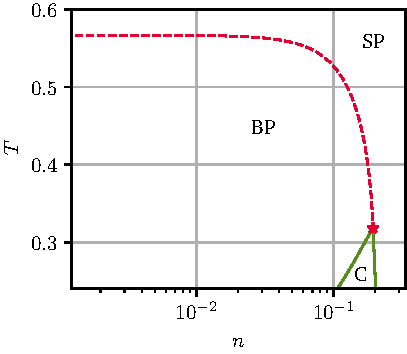
\includegraphics[]{gn/figures/gn_gl_ntPD.pdf}}% Graphics
	[]% Sublabels
	{%
		Phase diagram in the $n$-$T$-plane of the renormalized \gnm{} in the infinite-$N$ limit based on the \gle{}.
		With BP marking the symmetry-broken phase, SP marking the symmetry-restored phase, and C marking the region of phase coexistence associated with the first-order phase transition.
		Note that we have plotted only down to $T=0.25$ since the \gle{} only gives meaningful results for the first-order phase transition in the vicinity of the critical point, \cf{} \cref{fig:GNGLcompS} for a detailed plot of the analogous situation in the $\mu$-$T$-plane.
	}%Caption
	{fig:gn_gl_ntPD}%Label